\titre{Etude de points critiques et d'ue ligne de niveau}
\theme{calcul différentiel}
\auteur{}
\organisation{AMSCC}
\contenu{

\texte{ 	Une usine produit deux types de matériaux, que l'on note respectivement $A$ et $B$. Si elle produit $x$ kg de type $A$ et $y$ de type $B$ sur une semaine, le coût total hebdomadaire de production est 
$$c(x,y) = 600+200x+200y-2x^2y$$
%$$c(x,y) = 200x+200y+10xy-0.01x^2-0.01y^2+100$$
En pleine capacité, la production totale sur une semaine peut atteindre au maximum 30 kg. Dans cette modélisation, le coût peut être négatif.  }

\begin{enumerate}
	\item \question{ Décrire et représenter graphiquement le domaine de définition de la fonction $c$. }
	\reponse{D'après les informations données ici, on travaille sous la condition que $x+y \leq 30$ et $x\geq 0$, $y \geq 0$. Ces trois conditions définissent un triangle dans $\R^2$ :
		\begin{center}
			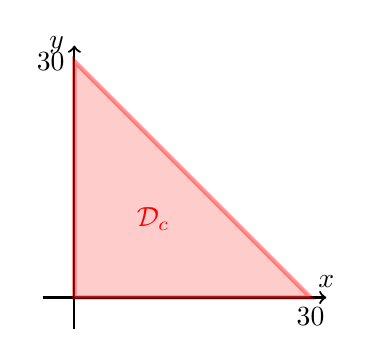
\begin{tikzpicture}
				\draw[thick,->] (-0.4,0)--(3.2,0)node[above] {$x$ };
				\draw[thick,->] (0,-0.4)--(0,3.2)node[left] {$y$};
				\draw[ultra thick, color=red, fill=red!50, opacity=0.4] (0,0)--(3,0)--(0,3) -- cycle;
				\draw[red] (1,1) node{$\mathcal{D}_c$};
				\draw (3,0) node[below]{$30$};
				\draw (0,3) node[left]{$30$};
			\end{tikzpicture}
		\end{center}	
		
	}
	\item \question{ Faire une recherche de minimum local à l'intérieur du domaine du définition. }
	\reponse{La fonction $c$ est polynomiale donc de classe $\mathcal{C}^{\infty}$ sur $\R^2$. On fait une recherche de points stationnaires $(x,y) \in \mathcal{D}_c$ :
		\begin{align*}
			\begin{cases}
				\frac{\partial c}{\partial x}(x,y) = 0\\
				\frac{\partial c}{\partial y}(x,y) =0
			\end{cases}
			\Leftrightarrow
			\begin{cases}
				200-4xy = 0\\
				200-2x^2 =0
			\end{cases}		
			\Leftrightarrow
			\begin{cases}
				x = 10\\
				y = 5
			\end{cases}			
		\end{align*}
		Un unique point stationnaire (point critique) est trouvé, il reste à étudier sa nature en regardant les conditions d'ordre 2. 
		
		$$Hess_c(x,y)=\begin{pmatrix} 
			\frac{\partial^2 c}{\partial x^2}(x,y) = -4y & \frac{\partial^2 c}{\partial x \partial y}(x,y) = -4x \\
			\frac{\partial^2 c}{\partial y \partial x}(x,y) = -4x & \frac{\partial^2 c}{\partial y^2}(x,y) = 0 &
		\end{pmatrix}$$
		Son déterminant est $0-16x^2$ donc pour le point stationnaire, $x=10$ et le déterminant vaut $-1600 <0$. D'après le cours, cette fonction présente un point selle en $(10,5)$. C'est le seul point stationnaire, il n'y a donc pas de minimum local pour la fonction $c$ à l'intérieur de $\mathcal{D}_c$. 
	}
	\item \question{ En substituant une variable en fonction d'une autre, étudier la fonction $c$ au bord du domaine. }
	\reponse{On travaille sur le bord :
		\begin{itemize}
			\item $x=0$ : on ne produit que du type B, le coût total est $c(0,y)=600+200y$, cette quantité est maximale pour $y=30$ et vaut $c(0,30)=6600$, cette quantité est minimale pour $y=0$ et vaut $c(0,0)=600$.
			\item $y=0$ : on ne produit que du type A, le coût total est $c(x,0)=600+200x$, cette quantité est maximale pour $x=30$ et vaut $c(300,0)=6600$, cette quantité est minimale pour $x=0$ et vaut $c(0,0)=600$.
			\item $x+y=300$ : 
			\begin{itemize}
				\item \textbf{Méthode par substitution} : on remplace $y$ par $30-x$ et on étudie la fonction d'une variable $f(x)=c(x,30-x) = 6600-60x^2+2x^3$ définie et dérivable sur $[0;30]$. On dérive : $f'(x) = 6x(x-20)$, on voit que $f'$ s'annule à l'intérieur du domaine en un seul point : $x_0 = 20$. On étudie la nature de ce point critique avec la dérivée seconde : 
				$f''(x_0) = 120 >0$, en déduit qu'il s'agit d'un minimum. 
				
				Pour minimiser le coût, l'usine doit produire 20 kg de type A et 10 kg de de type B pour un coût hebdomadaire de $c(20,10) = -1400$.  \\
				\textbf{Méthode du Lagrangien} : le lagrangien s'écrit ici $L(x,y,\lambda) = c(x,y)-\lambda(x+y-30) = 600+200x+200y-2x^2y-\lambda(x+y-30)$. On cherche son maximum par recherche de points critiques sur l'ensemble $]0;30[\times]0;30[\times\R$. On résout :
				\begin{align*}
					\begin{cases}
						\frac{\partial L}{\partial x}(x,y,\lambda) = 0\\
						\frac{\partial L}{\partial y}(x,y,\lambda) = 0\\
						\frac{\partial L}{\partial \lambda}(x,y,\lambda) = 0\\
					\end{cases}
					\Leftrightarrow
					\begin{cases}
						200-4xy-\lambda = 0\\
						200-2x^2-\lambda = 0\\
						30-x-y = 0\\
					\end{cases}
					\Leftrightarrow
					\begin{cases}
						200-4x(30-x)-(200-2x^2) = 0\\
						\lambda = 200-2x^2\\
						y= 30-x\\
					\end{cases} \\
					\Leftrightarrow \begin{cases}
						x = 20\\
						\lambda = -1600\\
						y= 10\\
					\end{cases}
				\end{align*}
				Reste à vérifier que ce point réalise le maximum du lagrangien en étudiant les conditions de second ordre : on évalue $\Delta(x,y,\lambda) = \frac{\partial^2 L}{\partial x^2}(x,y,\lambda)\frac{\partial^2 L}{\partial y^2}(x,y,\lambda) - \left(\frac{\partial^2 L}{\partial x \partial y}(x,y,\lambda) \right)^2 = -16x^2<0$. D'après le cours, on ne peut pas conclure directement. On doit donc étudier le signe de $c(x,y)-c(20,10)$ au voisinage de $(20,10)$ le long de la ligne d'équation $x+y=300$ : on étudie donc $d(h,k)=c(20+h,10+k)-c(20,10)$ compte tenu de la contrainte que $10+h+20+k = 30 \iff h=-k$. On étudie donc $d(h,-h) =  2h^2(30+h) \geq 0$. Cela garantit que $c(20,10)$ est bien un minimum de la fonction $c$.
			\end{itemize}
		\end{itemize}
		
	}
\end{enumerate}}
